\documentclass[12pt]{beamer}

\usetheme{Oxygen}
\usepackage{thumbpdf}
% \usepackage{wasysym}
% \usepackage{ucs}
\usepackage{multicol}
\usepackage{minted}
\usepackage[utf8x]{inputenc}
\usepackage{pgf,pgfarrows,pgfnodes,pgfautomata,pgfheaps,pgfshade}
\usepackage{verbatim}

\pdfinfo
{
  /Title       (MongoDB - Taller)
  /Creator     (TeX)
  /Author      (Miguel Angel Gordian Sanchez)
}


\title{MongoDB}
\subtitle{Taller basico}
\author{Miguel Angel Gordian}
\institute{Aztli}
\date{\today}

%Elimina los simbolos de navegacion
 \setbeamertemplate{navigation symbols}{}

% Establece el footline
\setbeamertemplate{footline}{%
  \begin{beamercolorbox} [sep=1.5em,wd=\paperwidth,leftskip=0.5cm,rightskip=0.5cm]{footlinecolor}
    \insertshortauthor~|~\insertshorttitle
    \hfill
    
\includegraphics[scale=0.04]{Img/mongo-onwhite.png}

    \insertinstitute
    \hfill
    \insertframenumber/\inserttotalframenumber


  \end{beamercolorbox}%
}

\setbeamertemplate{section in toc}
{
\includegraphics[width=7pt,height=12pt]{Img/mongodb_hoja.png}
  \hspace*{0.7em}\inserttocsection}


\PrerenderUnicode{ó}


%%%%%%%%%%%%%%%%%%%%%%%%%%%%%%%%%%%%%%%%%%%%%%%%%%%%%%%%%%%%%%%%%%%%%%
%%%%%%%%%%%%%%%%%%%%%%%%%%%%%%%%%%%%%%%%%%%%%%%%%%%%%%%%%%%%%%%%%%%%%%

\begin{document}
% background del codigo
\definecolor{bg}{rgb}{0.90,0.90,0.90}

% Presentacion - diapositiva 1
{
  \setbeamertemplate{footline}{}
  \setbeamertemplate{headline}{}
  \frame{\titlepage}
}


\section*{Resumen}
\begin{frame}
  \frametitle{Resumen}
     \begin{multicols}{2}
  \tableofcontents[section=1,hidesubsections]
     \end{multicols}
\end{frame}

\AtBeginSection[]
{

    \frame<handout:0>
    {
      \frametitle{Resumen}
      \begin{multicols}{2}
        \tableofcontents[currentsection,hideallsubsections]
      \end{multicols}
    }

 
}

\AtBeginSubsection[]
{
  \frame<handout:0>
  {
    \frametitle{Resumen}
    \tableofcontents[sectionstyle=show/hide,subsectionstyle=show/shaded/hide]
  }
}

\newcommand<>{\highlighton}[1]{%
  \alt#2{\structure{#1}}{{#1}}
}

\newcommand{\icon}[1]{\pgfimage[height=1em]{#1}}



%%%%%%%%%%%%%%%%%%%%%%%%
% Inicio del contenido %
%%%%%%%%%%%%%%%%%%%%%%%%


\section{MongoDB}

\section*{¿Qué es MongoDB?}
\frame {
  \vfill
  \centering
  \highlighton{
    \usebeamerfont*{frametitle}MongoDB

    \usebeamerfont*{framesubtitle}La base de datos NoSQL
  }
  \vfill
}

\begin{frame}{Caracteristicas}
  \begin{itemize}
  \item[$\bullet$]<1-> Base de datos
    
  \item[$\bullet$]<2-> Orientada a documentos
    
  \item[$\bullet$]<3-> Alto rendimiento
    
  \item[$\bullet$]<4-> Open source
    
  \item[$\bullet$]<5-> Horizontally scalable
  \end{itemize}
\end{frame}


\begin{frame}[fragile]{Documentos}
  \begin{block}{Documentos}
    Esencialmente un documento es un array asociativo, los cuales son  estructuras de 
    datos que mantienen la informacion en la base de datos.
  \end{block}
  \vfill
  \begin{minted}[bgcolor=bg]{js+cheetah}
    {
      name: "mongo",
      type: "DB"
    }
  \end{minted} 
\end{frame}

\begin{frame}{Open source}
  \begin{itemize}
    \item[$\bullet$] Opensource

    \item[$\bullet$] Github

    \item[$\bullet$] Licencia AGPL

    \item[$\bullet$] Iniciado y patrocinado por 10gen

    \item[$\bullet$] Licencia comerciales

    \item[$\bullet$] Las contribuciones  son bienvenidas
  \end{itemize}
\end{frame}


\begin{frame}{Rendimiento}

  \begin{itemize}
  \item[$\bullet$] Escrito en C++

  \item[$\bullet$] Uso extensico de mapeo de memoria de archivos

  \item[$\bullet$] Sopoerte completo para indices primarios y secundarios

  \item[$\bullet$] Uso de bson para el manejo de los datos

  \item[$\bullet$] Modelos de documentos (menos trabajo)
  \end{itemize} 
\end{frame}

\begin{frame}{Horizontally Scalable}
  \begin{center}
    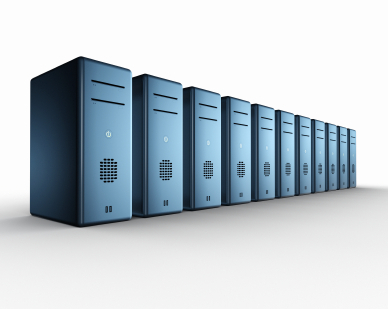
\includegraphics[scale=2]{Img/horizontal-scalability.jpg}    
  \end{center}
\end{frame}



\begin{frame}{Soporte completo}
  \begin{itemize}
  \item[$\bullet$] Consultas Ad hoc

  \item[$\bullet$] Versatilidad y potencia en consultas

  \item[$\bullet$] Soporte para operaciones geo-espaciales

  \item[$\bullet$] Soporte para gran variedad de lenguajes
    programacion.

  \item[$\bullet$] Schema flexible
  \end{itemize}
\end{frame}

\begin{frame}{Mongo Shell\footnote{Es solo javascript y un REPL}}
  \begin{center}
    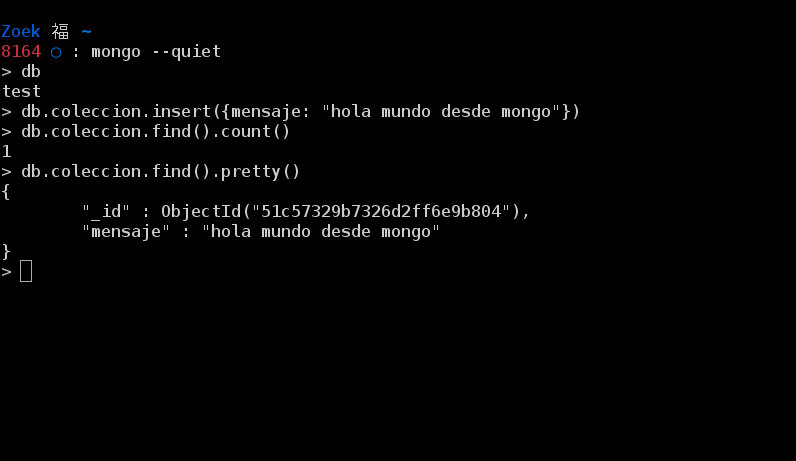
\includegraphics[scale=0.3]{Img/shell-mongo.png}    
  \end{center}
\end{frame}


\begin{frame}[fragile]{mongod}
  \begin{block}{mongod}
    Es el demonio para que maneja las peticiones de datas, el formato de los
    datos y el rendimiento de las operaciones en background.
  \end{block}

  Opciones por defecto:
  
  \begin{itemize}
      \item[$\bullet$] \textbf{/data/db} - Directorio de datos
      \item[$\bullet$] \textbf{27017} - Puerto de comunicación (usa tcp)
  \end{itemize}
\end{frame}


\begin{frame}[fragile]{Encedido/Apagado mongod}
  
  \begin{itemize}
    \item Encendido

    \begin{minted}[bgcolor=bg]{bash}
$ mongod --journal --dbpath=~mymongo/db \
         --logpath=~mymongo/logs/log.1
    \end{minted}
    
    \item Apagado
      \begin{minted}[bgcolor=bg]{bash}
$ mongod --shutdown
      
$ kill -2 <pid>  # SIGINT
$ kill -15 <pid> # SIGTERM
      \end{minted}
  \end{itemize}
\end{frame}

\section{CRUD}
\begin{frame}{¿Qué es el CRUD?}
  
  \begin{itemize}
  \item[$\bullet$]<1->  Creat - Insert

  \item[$\bullet$]<2->  Read - Find

  \item[$\bullet$]<3->  Update - Update

  \item[$\bullet$]<4->  Delete - Remove 
  \end{itemize}
\end{frame}

\begin{frame}[fragile]{Insert}
  
  \begin{itemize}
  \item Inserta un nuevo documento en la base de datos.

    \begin{minted}[bgcolor=bg]{js+cheetah}
db.<coleccion>.insert({clave: valor})
    \end{minted}
    
  \end{itemize}
\end{frame}


\begin{frame}[fragile]{Find}

  \begin{itemize}
  \item Busqueda de elementos.

    \begin{minted}[bgcolor=bg]{js+cheetah}
db.<coleccion>.findOne({clave: valor})
db.<coleccion>.find({clave: valor})
    \end{minted}
  \end{itemize}
\end{frame}

\renewcommand{\PYZdl}{\textdollar}

\begin{frame}[fragile]{Update}

  \begin{itemize}

    \item Actualizar uno o mas campos del documento
      \begin{minted}[bgcolor=bg]{js+cheetah}
db.<coleccion>.update({clave: valor}, 
   {$set: {nuevaclave: nuevovalor}})
         \end{minted}

       \item Sustituir el documento 
        \begin{minted}[bgcolor=bg]{js+cheetah}
db.<coleccion>.find({clave: valor})
         \end{minted}

         \item Eliminar un campo del documento
           \begin{minted}[bgcolor=bg]{js+cheetah}
db.<coleccion>.update({clave: valor}, 
    {$unset: {eleminarclave: 1}})
           \end{minted}
    
  \end{itemize}
\end{frame}
%$

\begin{frame}[fragile]{Remove}

  \begin{itemize}
    \item Eliminar documentos que concuerden con el documento pasado como parametro.

    \begin{minted}[bgcolor=bg]{js+cheetah}
db.<coleccion>.remove({clave: valor})
    \end{minted}
  \end{itemize}
\end{frame}

\begin{frame}[fragile]{Contar elemetos}

  \begin{itemize}
    \item Cuenta el numero de elementos devueltos a travez de una consulta.

    \begin{minted}[bgcolor=bg]{js+cheetah}
db.<coleccion>.find().count()
    \end{minted}
  \end{itemize}
\end{frame}

\begin{frame}[fragile]{Ordenacion}

  \begin{itemize}
    \item Ordenacion de la consulta en orden ascendente a travez del campo cualquiera.

    \begin{minted}[bgcolor=bg]{js+cheetah}
db.<coleccion>.find().sort({cualquiera: 1})
    \end{minted}

    \item Ordenacion de la consulta en orden descendente a travez del campo cualquiera.

    \begin{minted}[bgcolor=bg]{js+cheetah}
db.<coleccion>.find().sort({cualquiera: -1})
    \end{minted}

  \end{itemize}
\end{frame}

\begin{frame}[fragile]{Limitar}
  \begin{itemize}
    \item Evita los primeros N elementos.

    \begin{minted}[bgcolor=bg]{js+cheetah}
db.<coleccion>.find().skip(N)
    \end{minted}

    \item Limita la consulta a solo N elementos.

    \begin{minted}[bgcolor=bg]{js+cheetah}
db.<coleccion>.find().limit(N)
    \end{minted}

  \end{itemize}
\end{frame}

\section{Indexes}

\begin{frame}[fragile]{Crear Indice}
  Crear un indice es una operacion bloqueante que puede llegar a tomar
  mucho tiempo completarla, para ello se puede agregar la opcion 
  {background: true}, en las opciones.

  \begin{itemize}
  \item Crear un indice ascendente
    \begin{minted}[bgcolor=bg]{js+cheetah}
db.<coleccion>.ensureIndex({key: 1})
    \end{minted}

  \item Crear un indice ascendente
    \begin{minted}[bgcolor=bg]{js+cheetah}
db.<coleccion>.ensureIndex({key: -1})
    \end{minted}


    \item Crear un index geo-espacial
    \begin{minted}[bgcolor=bg]{js+cheetah}
db.<coleccion>.ensureIndex({locacion: "2d"})
    \end{minted}
  \end{itemize}
\end{frame}


\section{Aggregation}
\begin{frame}{Definición}
\
\begin{block}{Aggregation Framework}
  Provee una manera de calcular datos agregados, sin tener que usar map-reduce.
\end{block}
\end{frame}

\begin{frame}{Operaciones}
  
  \begin{itemize}
    \item \$project
    \item \$match
    \item \$limit
    \item \$skip
    \item \$unwind
    \item \$group
    \item \$sort
    \item \$geoNear    
    \end{itemize}
\end{frame}


\begin{frame}[fragile]{Ejemplo de documento}
  \begin{multicols}{2}
    \begin{itemize}
  \item Documento
    \begin{minted}[baselinestretch=1,fontsize=\scriptsize,bgcolor=bg]{js+cheetah}
{
  title : "this is my title" ,
  author : "bob" ,
  posted : new Date () ,
  pageViews : 5 ,
  tags : [ "fun" , "good", 
           "fun" ] ,
  comments : [
  { author :"joe" , 
    text : "this is cool" } ,
  { author :"sam" , 
    text : "this is bad" }
  ],
  other : { foo : 5 }
}
   \end{minted}

 \item Aggregation
     \begin{minted}[baselinestretch=1, fontsize=\scriptsize, bgcolor=bg]{js+cheetah}
db.articles.aggregate(
{ $project : {
    author : 1,
    tags : 1,
  } },
{ $unwind : "$tags" },
{ $group : {
    _id : { 
      tags : "$tags" },
    authors : { 
      $addToSet : "$author" }
  } }
);
\end{minted} 
      
    \end{itemize}
  \end{multicols}
\end{frame}

% \section{Limits}

\section{Permisos}
\begin{frame}[fragile]{Agregar usuario}
Usa db.addUser() para agregar docuemtnos a la coleccion system.users collection en la base de datos, la cual crea y mantiene las credecnciales en MongoDB.

\begin{minted}[bgcolor=bg]{js+cheetah}
db.addUser( { user: "<user>", 
              userSource: "<database>", 
              roles: [<roles>] } )
\end{minted}
\end{frame}

\begin{frame}[fragile]{roles}
\begin{multicols}{2}

  \begin{itemize}
    \item read

    \item readWrite

    \item dbAdmin

    \item userAdmin

    \item clusterAdmin

    \item readAnyDatabase

    \item readWriteAnyDatabase

    \item userAdminAnyDatabase

    \item dbAdminAnyDatabase
    
  \end{itemize}
\end{multicols}
\end{frame}


\begin{frame}[fragile]{mongod bypass}
Si no existen usuarios en la base de datos, se puede obtener todos los
privilegios al conectarse via localhost, para desabilitar bypass se inicia el
demonio de la siguiente manera.

\begin{minted}[bgcolor=bg]{js+cheetah}
mongod --setParameter enableLocalhostAuthBypass=0
\end{minted}
\end{frame}


\newcommand{\putlink}[1]{%
   \pgfsetlinewidth{1.4pt}%
   \pgfsetendarrow{\pgfarrowtriangle{4pt}}%
   \pgfline{\pgfxy(1,1)}{\pgfxy(#1,1)}
}


\begin{frame}
  \frametitle{Recursos}
  \framesubtitle{¿Donde continuar?}
  \begin{thebibliography}{10}

  \beamertemplatearticlebibitems

  \bibitem{Mongo-homepage}
    Mongo
    \newblock {\tt http://www.mongodb.org/}

  % \bibitem{Presentacion-slides}
  %   Mongo - taller
  %   \newblock {\tt http://www.kde.org/kdeslides/}

  \end{thebibliography}
\end{frame}

\frame{
  \vspace{2cm}
  {\huge ¿Preguntas?}

  \vspace{3cm}
  \begin{flushright}
    Miguel Angel Gordian

    \structure{\footnotesize{os.aioria@gmail.com}}
  \end{flushright}
}

\end{document}
